\chapter{Conception logicielle, refactoring et bonnes pratiques de développement}
    \section{Refactoring des précédents travaux}

        \cite{clean_code}

\begin{lstlisting}[caption={Exemple de fonction refactorisée}]
def get_input_parameters(input_parameters_file, input_parameters_row_index=-1):
    input_parameters_df = pd.read_csv(input_parameters_file)

    studied_building_name = input_parameters_df["building_name"].iloc[input_parameters_row_index]
    mode_pso = input_parameters_df["enable_parameters_optimization"].iloc[input_parameters_row_index]
    identification_starting_date = input_parameters_df["identification_starting_date"].iloc[input_parameters_row_index]
    identification_starting_hour = input_parameters_df["identification_starting_hour"].iloc[input_parameters_row_index]
    identification_ending_date = input_parameters_df["identification_ending_date"].iloc[input_parameters_row_index]
    identification_ending_hour = input_parameters_df["identification_ending_hour"].iloc[input_parameters_row_index]

    return studied_building_name, mode_pso, identification_starting_date, identification_starting_hour, identification_ending_date, identification_ending_hour\end{lstlisting}


        \begin{figure}[H]
            \centering
            \subfloat[Projet de 2023]{\fbox{
                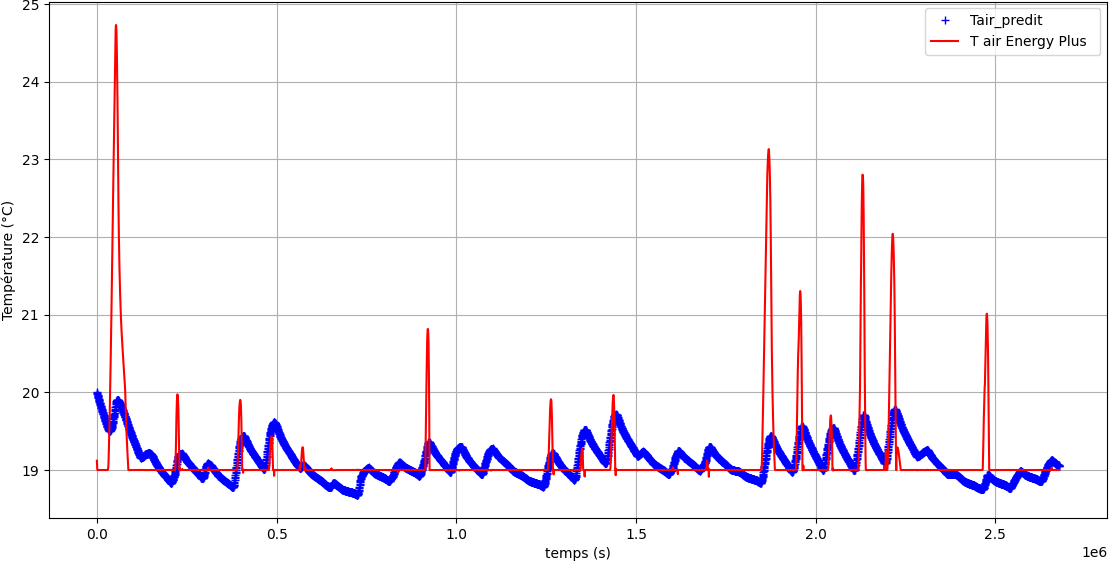
\includegraphics[width = 0.4\textwidth]{figures/diagrammes/courbes/TST_air_predit_VS_energyplus}}}\qquad
            \subfloat[Projet actuel]{\fbox{
                
\includegraphics[width = 0.4\textwidth]{figures/placeholder}}}\qquad
            \caption{Comparaison entre les sorties des deux programmes}
        \end{figure}

        \begin{table}[h!]
            \centering
            \begin{tabular}{lcc}
                \toprule
                \textbf{Critère} & \textbf{Projet de 2023} & \textbf{Projet actuel} \\
                \midrule
                Nombre de lignes totales &  &  \\
                Traitement des données &  &  \\
                Plus longue fonction &  &  \\
                Plus courte fonction &  &  \\
                Nombre de fonctions &  &  \\
                Noms de variables &  &  \\
                Arborescence de fichiers &  &  \\
                Fonctions implémentées vs fonctions de librairies &  &  \\
                Approche objet &  &  \\
                Gestion de projet (aucune VS Gitlab) &  &  \\
                Librairies utilisées &  &  \\
                \bottomrule
            \end{tabular}
            \caption{Comparaison qualitative et quantitative entre le projet de 2023 et le projet actuel}
        \end{table}


    \section{Évaluation qualitative des performances du projet}
        \subsection{Complexité des algorithmes appelés}
        \subsection{Outils retenus pour garantir la performance}
            \subsection{\texttt{uv} plutôt que \texttt{conda} ou \texttt{pip}}
            \subsection{Polars plutôt que Pandas}

                \begin{table}[h!]
                    \centering
                    \begin{tabular}{lcc}
                        \toprule
                        \textbf{Calcul lancé} & \textbf{Avec \texttt{Pandas}} & \textbf{Avec \texttt{Polars}} \\
                        \midrule
                        Couple Dataset-Modèle 1 &  &  \\
                        Couple Dataset-Modèle 2 &  &  \\
                        \bottomrule
                    \end{tabular}
                    \caption{Benchmark de performance entre \texttt{Pandas} et \texttt{Polars}}
                \end{table}
